
\documentclass[12pt,a4paper]{amsart}
% ukazi za delo s slovenscino -- izberi kodiranje, ki ti ustreza
\usepackage[slovene]{babel}
%\usepackage[cp1250]{inputenc}
\usepackage[T1]{fontenc}
\usepackage[utf8]{inputenc}
\usepackage{amsmath,amssymb,amsfonts}
\usepackage{url}
\usepackage{graphicx}
\usepackage{subcaption}
%\usepackage[demo]{graphicx}
%\usepackage[normalem]{ulem}
\usepackage[dvipsnames,usenames]{color}
\usepackage{hyperref}
\hypersetup{
     colorlinks   = true,
     citecolor    = gray
}

\graphicspath{ {./slike/} }
% ne spreminjaj podatkov, ki vplivajo na obliko strani
\textwidth 15cm
\textheight 24cm
\oddsidemargin.5cm
\evensidemargin.5cm
\topmargin-5mm
\addtolength{\footskip}{10pt}
\pagestyle{plain}
\overfullrule=15pt % oznaci predlogo vrstico


% ukazi za matematicna okolja
\theoremstyle{definition} % tekst napisan pokoncno
\newtheorem{definicija}{Definicija}[section]
\newtheorem{primer}[definicija]{Primer}
\newtheorem{opomba}[definicija]{Opomba}

\renewcommand\endprimer{\hfill$\diamondsuit$}


\theoremstyle{plain} % tekst napisan posevno
\newtheorem{lema}[definicija]{Lema}
\newtheorem{izrek}[definicija]{Izrek}
\newtheorem{trditev}[definicija]{Trditev}
\newtheorem{posledica}[definicija]{Posledica}


% za stevilske mnozice uporabi naslednje simbole
\newcommand{\R}{\mathbb R}
\newcommand{\N}{\mathbb N}
\newcommand{\Z}{\mathbb Z}
\newcommand{\C}{\mathbb C}
\newcommand{\Q}{\mathbb Q}

% ukaz za slovarsko geslo
\newlength{\odstavek}
\setlength{\odstavek}{\parindent}
\newcommand{\geslo}[2]{\noindent\textbf{#1}\hspace*{3mm}\hangindent=\parindent\hangafter=1 #2}

% naslednje ukaze ustrezno popravi
\newcommand{\program}{Finančna matematika} % ime studijskega programa: Matematika/Finan"cna matematika
\newcommand{\imeavtorja}{Eva Ozebek\\ Jan Kolenc} % ime avtorja
\newcommand{\imementorja}{prof. dr. Riste Škrekovski} % akademski naziv in ime mentorja
\newcommand{\naslovdela}{Minimum vertex cover}
\newcommand{\letnica}{2019} %letnica




\begin{document}

% od tod do povzetka ne spreminjaj nicesar
\thispagestyle{empty}
\noindent{\large
UNIVERZA V LJUBLJANI\\[1mm]
FAKULTETA ZA MATEMATIKO IN FIZIKO\\[5mm]
\program\ -- 1.~stopnja}
\vfill

\begin{center}{\large
\imeavtorja\\[2mm]
{\bf \naslovdela}\\[10mm]
Projekt v povezavi z OR\\[1cm]}

\end{center}
\vfill

\noindent{\large
Ljubljana, \letnica}
\pagebreak

\thispagestyle{empty}
\hypersetup{linkcolor = black}
\tableofcontents
\pagebreak

\section{Navodilo}


Define the Minimum vertex cover problem as an ILP and solve it for some examples. Also, solve the LP relaxation of this problem for the same cases. Note that its LP relaxation gives a solution that is at most twice bigger than the optimal one. Compare the sizes of both solutions on various graphs to verify this and determine experimentally by how much, in average, the LP relaxation solution is larger than the optimal one. Finally, present and implement a greedy algorithm and the one using the maximal matching described in the book below. Test the sizes of these three solutions. Try to determine for how large graphs each of these algorithms is tractable.

\newpage
\section{Uvod}

Najina naloga je, da problem najmanjšega vozliščnega pokritja predstaviva kot problem ILP, LP relaksacije ter požrešnega algoritma. Pri tem bova algoritme preverila za 1000 različnih primerov grafov, ki imajo naključno med 5 in 100 vozlišč in naključnih povezav. Primerjala bova rezultate različnih algoritmov, kjer naju bo še posebej zanimala velikost rešitve oz. v najinem primeru moč vrnjene množice.
Najine algoritme bova testirala na podatkih, ki jih bova generirala sama.

\hspace*{\fill} % it's important not to leave blank lines before and after this command
\\
Problem \textit{najmanjšega vozliščnega pokritja}  je eden izmed osnovnih problemov pokrivanja. Kot pove že ime samo, je problem definiran s pomočjo teorije grafov. Gre za pokrivanje povezav grafa z vozlišči, t.j. za iskanje najmanjše podmnožice vozlišč grafa, ki vsebuje vsaj eno krajišče vsake povezave grafa.


\hspace*{\fill} % it's important not to leave blank lines before and after this command
\\
Problem najmanjšega vozliščnega pokritja, ki je eden izmed zahtevnejših optimizacijskih problemov iz teorije grafov, spada v kategorijo NP-težkih problemov. Verjetnost, da je mogoče optimalno rešitev zanj najti v polinomskem času, je zelo majhna, obstaja pa več načinov za iskanje približka optimalne rešitve. 

\hspace*{\fill} % it's important not to leave blank lines before and after this command
\\
Pri programiranju in pisanju algoritma sva se odločila za program Sage, saj je le-ta za najino nalogo najbolj primeren.

\newpage

\begin{figure*}[ht]
\centering
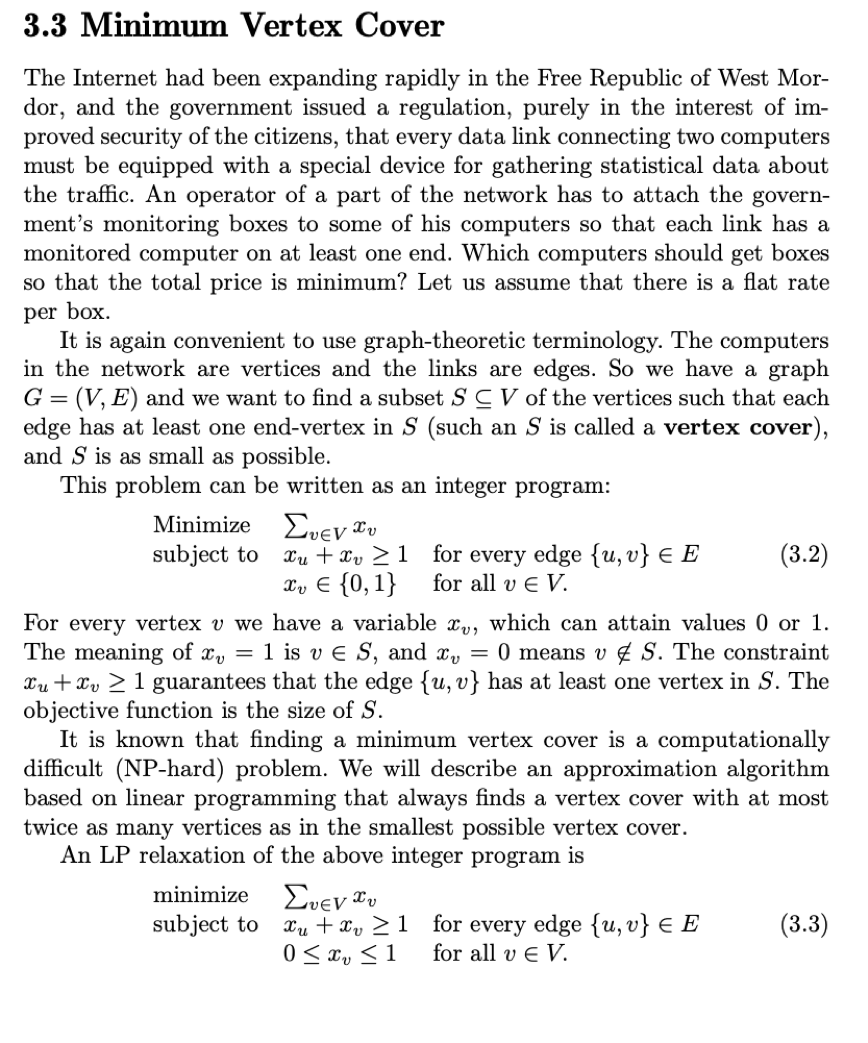
\includegraphics[width=1\textwidth]{Picture1.png}
\end{figure*}

\newpage

\begin{figure*}[ht]
\centering
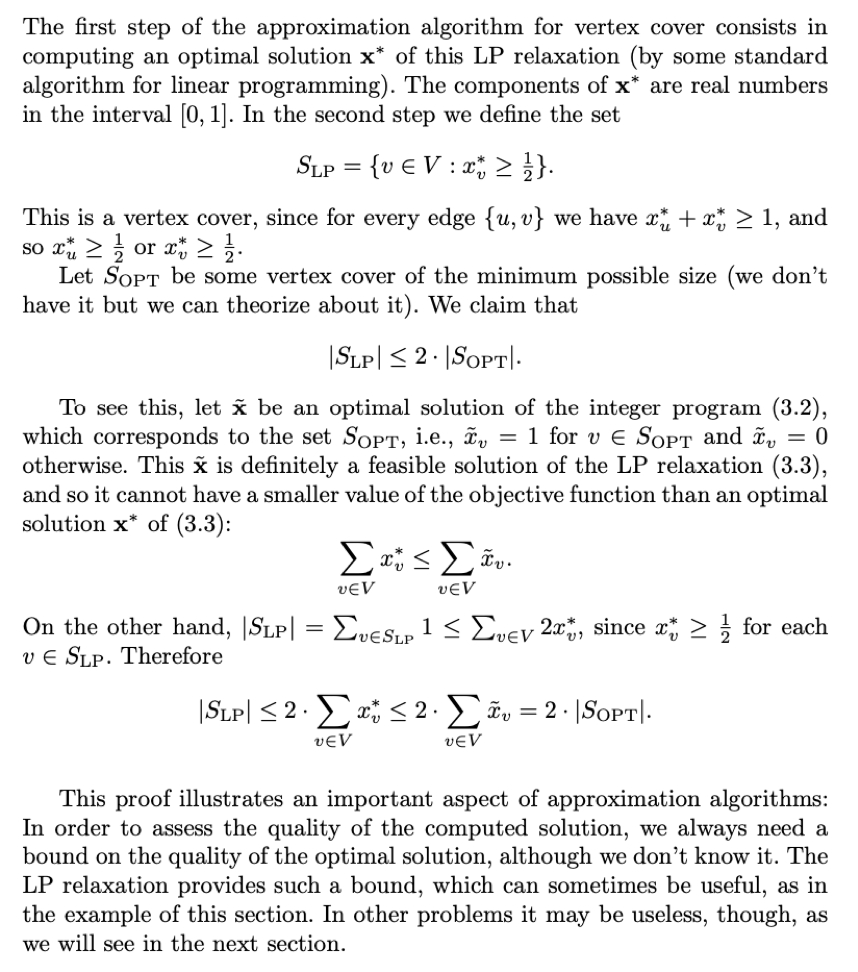
\includegraphics[width=1\textwidth]{Picture2.png}
\end{figure*}


\newpage

\begin{figure*}[ht]
\centering
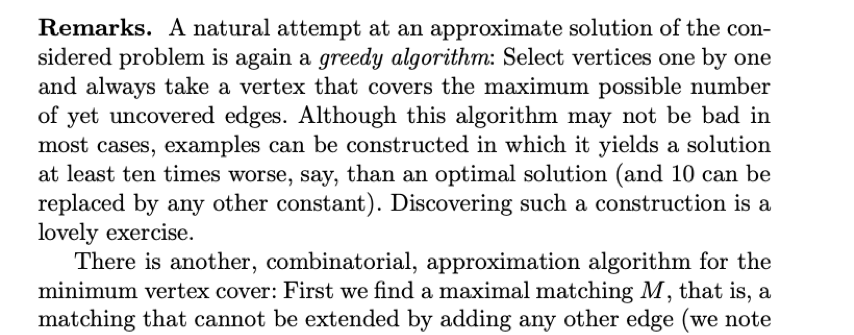
\includegraphics[width=1\textwidth]{Picture3.png}
\end{figure*}

\begin{figure*}[ht]
\centering
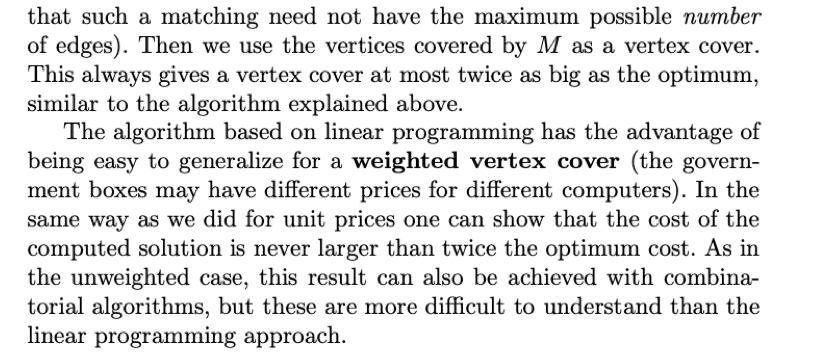
\includegraphics[width=1\textwidth]{Picture4.png}
\end{figure*}

%---------------------OPIS DELA- SCREENSHOTI --------------------

\newpage

\section{Opis dela}
\

\subsection{Generiranje grafov}
\
\\
\\
Najprej sva definirala funkcijo testiranje, ki vzame argumente \textit{a} (število različnih velikosti grafov), \textit{b} (število grafov iste velikosti), \textit{c} (največje možno število vozlišč), kar bomo uporabili pri generiranju grafov. Funkcija si na začetku shrani tudi 3 števce in sicer: koliko grafov smo že pregledali, seštevek koeficientov razlik - razlika velikosti rešitev algoritmov ILP in LP ter razlika velikosti rešitev algoritmov greedy in max matching. 




\begin{figure*}[ht]
\centering
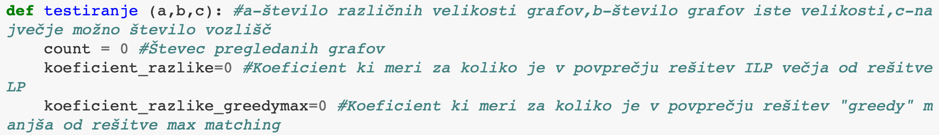
\includegraphics[width=1\textwidth]{Screen2.png}
\end{figure*}


 \hspace*{\fill} % it's important not to leave blank lines before and after this command
\\
Ko izžrebamo število vozlišč moramo še 10x žrebati število povezav. Generirala sva naključno število vozlišč in povezav, kjer sva število povezav morala omejiti (da ne presegajo števila povezav polnega grafa na n vozliščih (\textit{st\_vozlisc})), od tu izraz \textit{st\_vozlisc*(st\_vozlisc - 1)/2}. Ko se vozlišča in povezave naključno izberejo, na vsakem izmed 1000 korakov dobimo graf na katerem uporabljamo algoritme.


\begin{figure*}[ht]
\centering
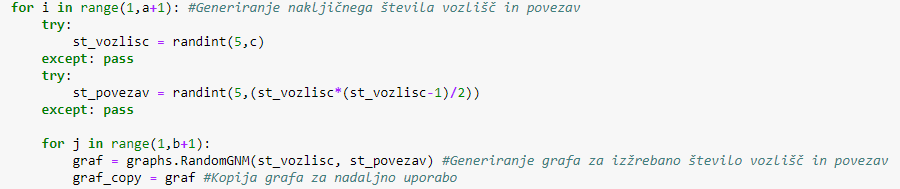
\includegraphics[width=1\textwidth]{Screen3.png}
\end{figure*}

\newpage

\subsection{Požrešni algoritem in algoritem maximum matching}
\
\\
\\
Definirala sva požrešni algoritem, ki sledi reševanju problemov lokalno optimalne izbire na vsaki stopnji, z namenom poiskati globalni optimum. Le-ta vsakič vzame vozlišče z največ povezavami in ta vozlišča shranjuje v seznam. 

 \hspace*{\fill} % it's important not to leave blank lines before and after this command
\\
Torej, ko imamo vozlišče z največ povezavami, te povezave odstranimo in to ponavljamo tako dolgo, dokler v grafu ni več nobenih povezav. Ta izbrana vozlišča so vertex cover. Kot lahko opazimo je naša rešitev seznam, dolžina seznama pa predstavlja velikost rešitve. 

 \hspace*{\fill} % it's important not to leave blank lines before and after this command
\\
Hkrati sva uporabila implementiran algoritem za maximum matching, ki nam vrne število povezav, zato na koncu rešitev pomnožimo z 2, saj nas zanima število vozlišč. 

\begin{figure*}[ht]
\centering
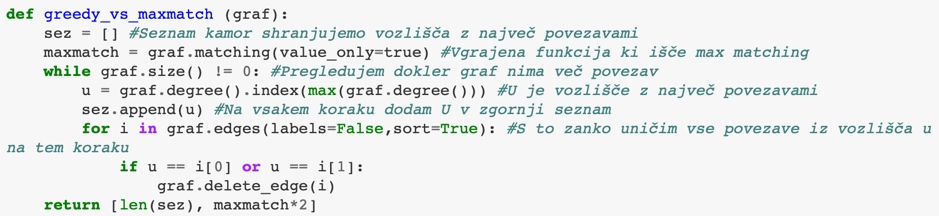
\includegraphics[width=1\textwidth]{Screen1.png}
\end{figure*}




\subsection{Celoštevilski linearni program}
\
\\
\\
Ko imamo generiran graf, na njem rešimo ILP in LP ter uporabimo funkcijo \textit{greedy\_vs\_maxmatch}.

 \hspace*{\fill} % it's important not to leave blank lines before and after this command
\\
ILP (\textit{integer linear program}) uporablja samo cela števila na zaprtem intervalu od 0 do 1, zato nastavimo \textit{binary = True}. Z \textit{set\_objective} določimo kaj želimo maksimizirati pri linearnih programih, v najinem primeru je to seštevek vrednosti prirejenih vozliščem. 

 \hspace*{\fill} % it's important not to leave blank lines before and after this command
\\
Nato omejitve (\textit{add\_constraints}) nastavimo tako, da je vsaka povezava v grafu šteta vsaj enkrat. Nato pa na vozlišča zapišemo vrednosti, ki jih jim je priredil ILP. Končno rešitev - torej vozlišča vsebovana v pokritju in velikost rešitve, bova prikazala kasneje. 


\begin{figure*}[ht]
\centering
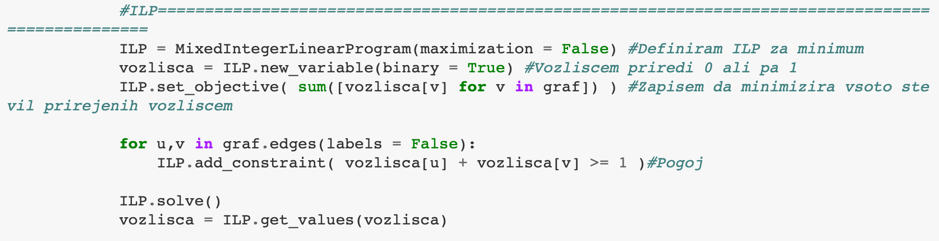
\includegraphics[width=1\textwidth]{Screen4.png}
\end{figure*}

\newpage

\subsection{Relaksacija celoštevilskega na linearni program}
\
\\
\\
Tukaj se ne ukvarjamo več s celimi števili, zato nastavimo \textit{real = True}. Realna števila sva omejila na interval od 0 od 1, nastavila sva iste pogoje in enak objective.

 \hspace*{\fill} % it's important not to leave blank lines before and after this command
\\
Ker uporabimo pogoj da mora biti vsota vozlišč večja ali enaka ena, zato vemo da mora biti posamezno vozlišče večje ali enako eni polovici. 

 \hspace*{\fill} % it's important not to leave blank lines before and after this command
\\ 
 Tudi tukaj bova rezultate in ugotovitve prikazala v naslednjem razdelku. 


\begin{figure*}[ht]
\centering
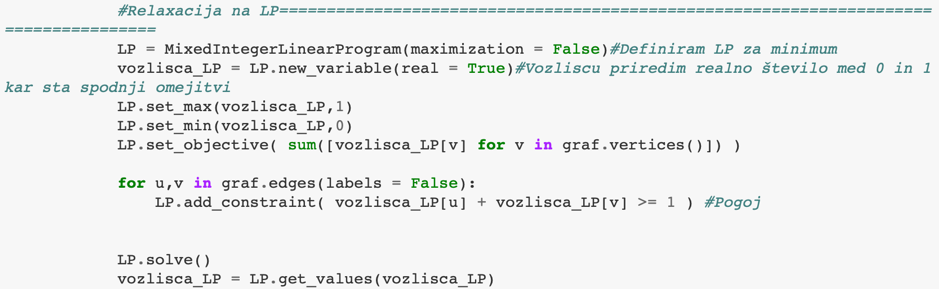
\includegraphics[width=1\textwidth]{Screen5.png}
\end{figure*}


\newpage

\subsection{Rezultati funkcij}
\
\\
\\
Na tej točki upoštevama funkcijo \textit{greedy\_vs\_maxmatch}, ki sva jo definirala zgoraj. Print vrne velikosti rešitev (greedy in maximum matching) hkrati, ter velikosti rešitev LP in ILP.

 \hspace*{\fill} % it's important not to leave blank lines before and after this command
\\ 
Potem primerjamo velikosti rešitev greedy in maximum matching, da vidimo za koliko krat je rešitev greedy manjša od velikosti rešitve maximum matching ter koeficient prištejemo k števcu za ta dva algoritma. Postopek ponovimo še za ILP in LP. 

 \hspace*{\fill} % it's important not to leave blank lines before and after this command
\\ 
Na koncu pa nama funkcija vrne povprečne koeficiente za oba para algoritmov.


\begin{figure*}[ht]
\centering
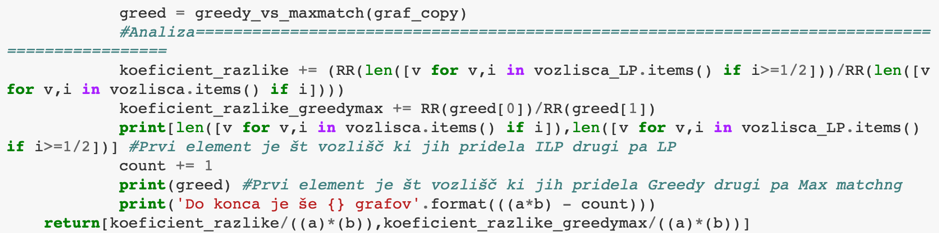
\includegraphics[width=1\textwidth]{Screen6.png}
\end{figure*}




\newpage



\section{Zaključek}

V najini analizi sva se, kot omenjeno že prej, osredotočila na 1000 primerov, ki sva jih generirala sama. Najprej sva definiranim grafom naključno izbrala med 5 in 100 vozlišč, nato pa dodala še naključne povezave.

\hspace*{\fill} % it's important not to leave blank lines before and after this command


Tekom analize sva uporabljala sledeče algoritme:
\begin{itemize}
\item ILP
\item LP
\item Požrešni algoritem
\item Maximal matching

 \end{itemize}

 \hspace*{\fill} % it's important not to leave blank lines before and after this command



\begin{figure*}[ht]
\centering
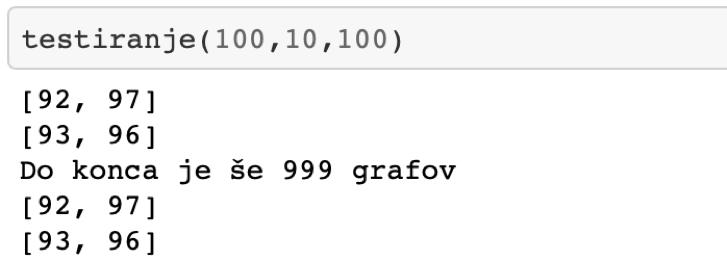
\includegraphics[width=.6\textwidth]{Screen7.png}
\end{figure*}


\begin{figure*}[ht]
\centering
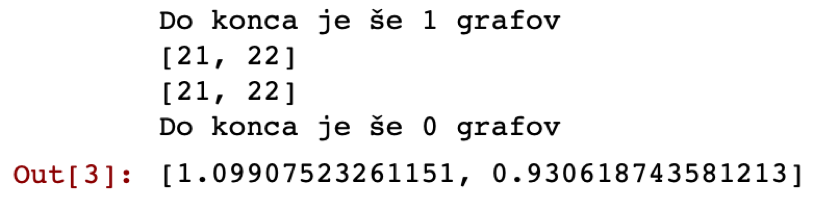
\includegraphics[width=.7\textwidth]{Screen8.png}
\end{figure*}

Kot vidimo zgoraj, sva opravila testiranje, kjer sva ugotovila, da je velikost rešitve LP v povprečju za 9,908\% večja od velikosti rešitve ILP. Prav tako pa sva ugotovila tudi, da je velikost rešitve maximum matching za 7,458\% večja od velikosti rešitve greedy.

\newpage


\begin{figure*}[ht]
\centering
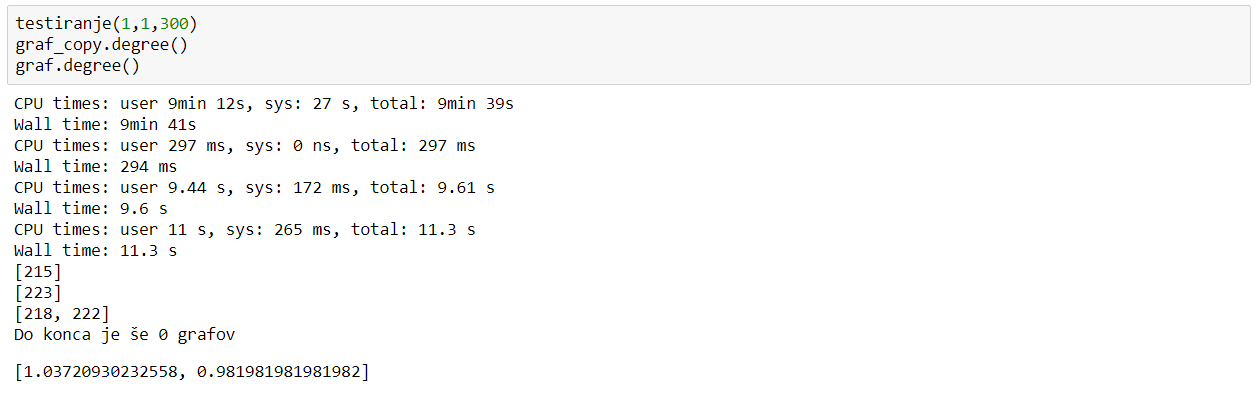
\includegraphics[width=1\textwidth]{Screen9.png}
\end{figure*}

 \hspace*{\fill} % it's important not to leave blank lines before and after this command
\\ 
Zanimalo naju je, koliko časa za velike grafe porabijo zgoraj opisani algoritmi. Za grafe do velikosti 50 vozlišč so bile razlike le v sekundah, kot pa vidimo na zgornjem primeru, kjer je bilo več kot 220 vozlišč, pa sta se časa reševanja ILP in LP razlikovala že za skoraj 10 minut. 

 \hspace*{\fill} % it's important not to leave blank lines before and after this command
\\ 
Pri algoritmih greedy in maximum matching ni bilo velikih razlik. Greedy je porabil 1,7 sekunde, maximum matching pa 9,6 sekunde. 

 \hspace*{\fill} % it's important not to leave blank lines before and after this command
\\ 
Kljub temu, da ILP problem rešuje največ časa, nam da najbolj točno rešitev, torej se lahko na podlagi velikosti grafa in zahtevane natančnosti odločimo za uporabo najbolj ustreznega algoritma za dan primer.

 \hspace*{\fill} % it's important not to leave blank lines before and after this command
\\ 
Za grafe, ki imajo do 200 vozlišč bi priporočala ILP, za večje grafe pa gotovo uporabo LP algoritma. 



\newpage
\begin{thebibliography}{}


\bibitem{teorija}
J.~Matoušek in B.~Gartner, \emph{Understanding and Using Linear Programming}


\bibitem{teorija}
 J.~Mihelič, \emph{Algoritem za problem najmanjšega vozliščnega pokritja}, [ogled 18.~11.~2019], dostopno na \url{https://www.researchgate.net/publication/308929074_Algoritmi_za_problem_najmanjsega_vozliscnega_pokritja?fbclid=IwAR0n6CzQluY3ZFM6g2-yQ_fPLnUiT8zrb78S_o3VUwjmf7F-_DNQzxHVqb0}




\end{thebibliography}{}

\end{document}
